\documentclass{report}
\usepackage{graphicx}
\begin{document}
\section*{Efectos de Audio}
\section*{Reverberaci\'{o}n}

\subsection*{Eco Simple}
Este efecto se puede implementar con el siguiente filtro, que adiciona a la se\~{n}al original una copia atenuada y retardada de la misma.
$$y(n)=x(n)+ax(n-D)$$
El retardo D representa el tiempo de viaje de la se\~{n}al ida y vuelta desde la fuente hasta una pared. El coeficiente $a$ es una medida de las pérdidas por reflexión y propagación ($|a|<1$).
La funci\'{o}n transferencia y respuesta al impulso de este filtro ser\'{a}:
$$H(z)=1+az^{-D}$$
$$h(n)=\delta(n)+a\delta(n-D)$$
Su diagrama en bloques es el que se muestra en siguiente figura

\begin{figure}[h]
  \centering
    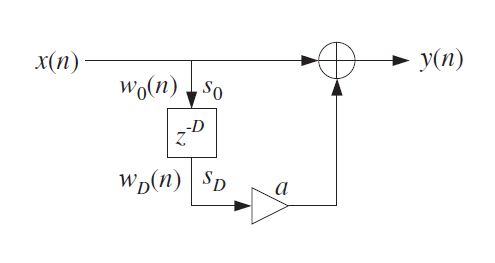
\includegraphics[scale=1]{imagenes/diag_eco_simple.png}
  \caption{ Diagrama en bloques del eco simple}
  \label{fig:SI}
\end{figure}

Dicho filtro actúa como un filtro comb FIR cuya respuesta de frecuencia muestra picos en
múltiplos de la frecuencia fundamental $f1 = \frac{f_s}{D}$.

Para su implementaci\'{o}n en C++, se utiliz\'{o} un buffer circular donde se iban guardando las D muestras anteriores a la muestra actual. 

\subsection*{Reverberador Plano}
En esta subsecci\'{o}n analizaremos como la suma de un número infinito de ecos sucesivos imita la naturaleza reverberante
de una habitación y da lugar a un filtro comb IIR. 

La suma de infinitos ecos sucesivos se expresa como:
$$y(n)=x(n)+ax(n-D)+a^{2}x(n-2D)+...$$
Cuya respuesta al impulso y funci\'{o}n transferencia esta dada por:
$$h(n)=\delta(n)+a\delta(n-D)+a^{2}\delta(n-2D)+...$$
$$H(z)=1-az^{-D}+a^2z^{-2D}+...$$
Que puede ser sumado por la serie geométrica en la forma:
$$H(z)=\frac{1}{1-az^{-D}}$$
Y podemos reescribir a $y(n)$ como:
$$y(n)=ay(n-D)+x(n)$$
El diagrama en bloques de este efecto es el siguiente:
\begin{figure}[h]
  \centering
    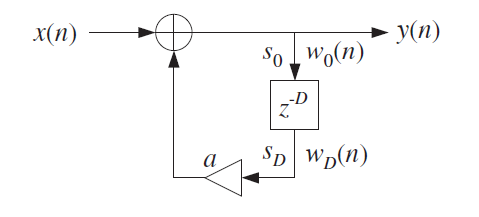
\includegraphics[scale=1]{imagenes/diag_eco_plano.png}
  \caption{ Diagrama en bloques del reverberador plano}
  \label{fig:SI}
\end{figure}

Para su implementaci\'{o}n en C++, al igual que el caso anterior, se utiliz\'{o} un buffer circular de tamaño 2*D que conten\'{i}a las D salidas anteriores a la actual a izquierda y derecha.

\subsection*{Flanger}
Se pueden crear efectos de audio más interesantes, como flanging,
permitiendo que D varíe en el tiempo de la forma: 
$$y(n)=x(n)+ax(n-d(n))$$
El efecto flanger se genera variando peri\'{o}dicamente el retardo $d(n)$ entre 0 y 10ms con una frecuencia baja, como 1Hz. Por ejemplo, un retraso que var\'{i}a sinusoidalmente entre los l\'{i}mites $0{\leq}d(n){\leq}D$ de la forma:
$$ d(n)= delay + rango .  sen(2{\pi}nF_d )$$
donde $d(n): [0-10ms]$ y $F_d[ciclos/muestra]{\sim}1Hz$

A continuaci\'{o}n se muestra el diagrama en bloques y la respuesta en frecuencia de este efecto.

\begin{figure}[h]
  \centering
    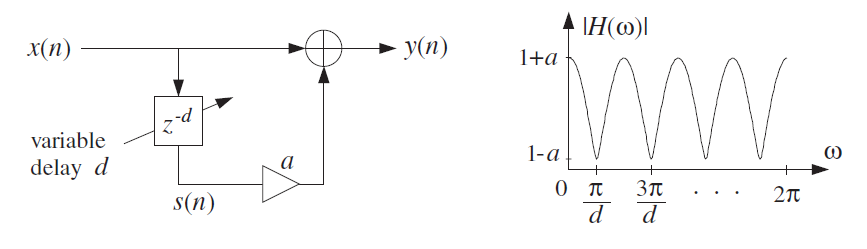
\includegraphics[scale=1]{imagenes/diag_flang.png}
  \caption{ Diagrama en bloques y respuesta en frecuencia del flanger}
  \label{fig:SI}
\end{figure}


Los picos de la respuesta en frecuencia del filtro comb variable en el tiempo ocurren en m\'{u}ltiplos de $\frac{f_s}{d}$ y sus notch en m\'{u}ltiplos impares de $\frac{f_s}{2d}$. Estos barren hacia arriba y hacia abajo el eje de frecuecnia, lo que dar\'{a} como resultado el sonido caracter\'{i}stico del flanger.

El parametro que controla la profundidad de los notch es $a$. En unidades de [radianes/muestra], los notch ocurren en m\'{u}ltiplos impares de $\frac{\pi}{d}$

Para la implementaci\'{o}n en C++, utilizamos un buffer circular de tamaño [2*(delay + range)] ya que el retardo m\'{a}ximo que puedo tener es la suma del delay y el range. En este buffer fueron guardadas las entradas retardadas. 

Otro detalle a tener en cuenta respecto al c\'{o}digo, es que debimos castear a int cada retardo $d(n)$ 

\subsection*{Reverberaci\'{o}n allpass}
Los picos en el espectro del filtro de reverberaci\'{o}n plano tiende a acentuar las frecuencias de la señal de entrada que estan cerca de las frecuencias pico. Para evitar lo antes descripto, Schroeder propuso una versi\'{o}n allpass de un reverberador plano. A continuaci\'{o}n se detallan sus caracteristicas: 
$$H(z)=\frac{-a+z^{-D}}{1-az^{-D}}$$
$$y(n)=ay(n-D)-ax(n)+x(n-D)$$
\begin{figure}[h]
  \centering
    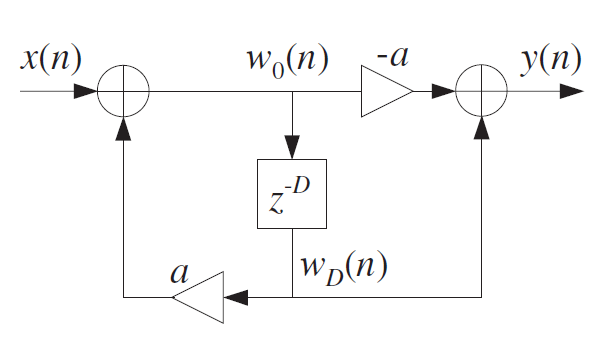
\includegraphics[scale=0.75]{imagenes/diag_allpass.png}
  \caption{ Diagrama en bloques del reverberador allpass}
  \label{fig:SI}
\end{figure}

Para la implementaci\'{o}n en C++, debieron utilizarse dos buffers circulares, uno para almacenar las entradas retardadas y otro para las salidas retardadas. 


\subsection*{Reverberador completo}
Para generar efectos de reverberaci\'{o}n m\'{a}s realistas pueden combinarse bloques de reverberaciones planas y allpass. El reverberador de Schroeder consiste en varios bloques de reverberaciones planas conectadas en paralelo, seguidas de bloques de reverberaciones allpass en cascada.
A continuaci\'{o}n se muestra un diagrama de lo antes descripto.

\begin{figure}[h]
  \centering
    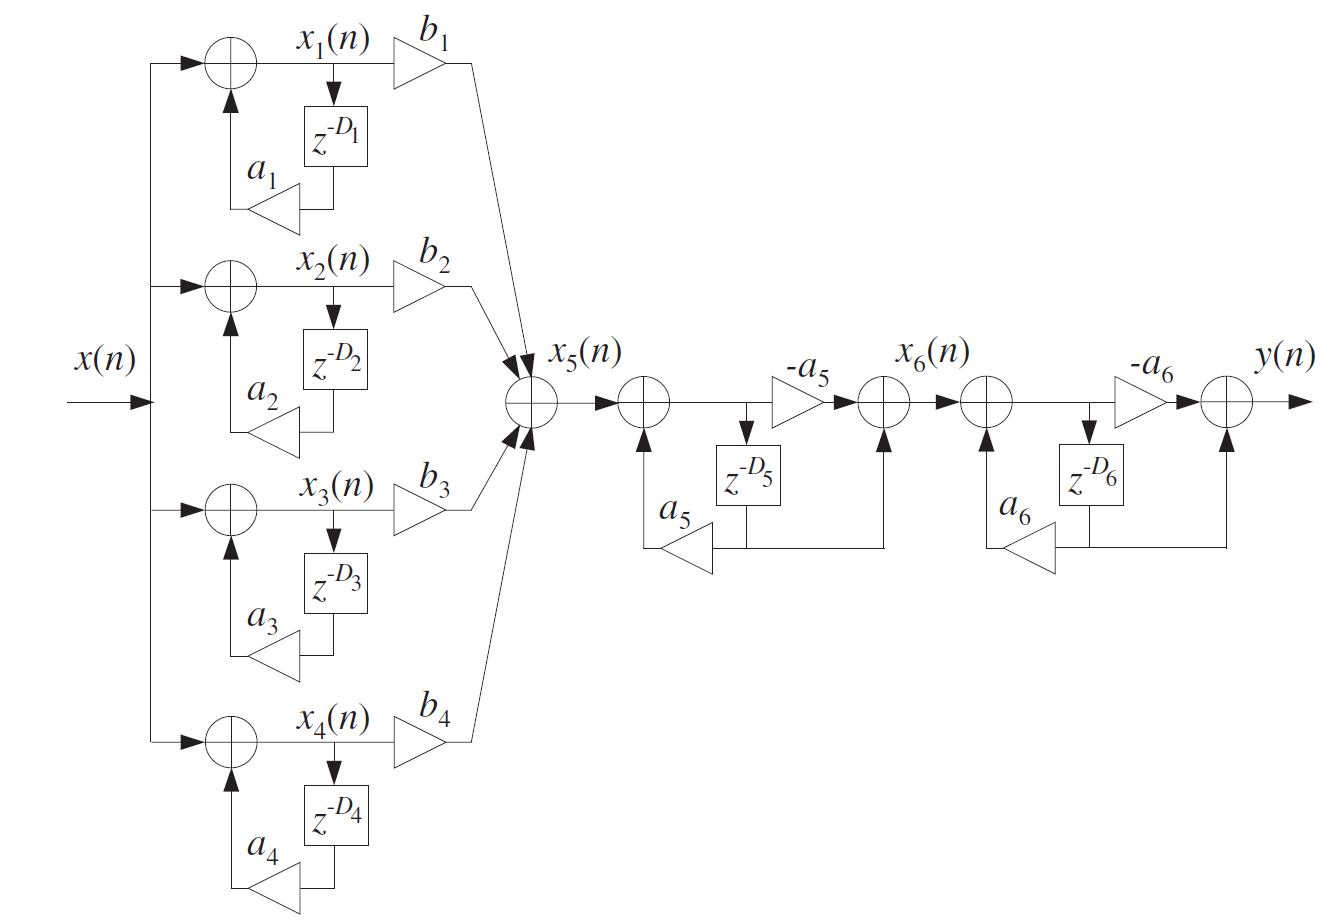
\includegraphics[scale=0.75]{imagenes/diag_sh.png}
  \caption{ Diagrama en bloques del reverberador completo}
  \label{fig:SI}
\end{figure}


  Para comprobar la funcionalidad de este efecto, se implement\'{o} en C++ una versi\'{o}n sencilla de reverberador Schroeder. El mismo consta de tres reverberadores planos en paralelo cuyos par\'{a}metros de entrada son $D1$, $D2$ y $D3$ (retardos, distintos para cada bloque) y  $a$ (coeficiente, el mismo para los tres bloques). Seguido se conecta un \'{u}nico reverberador allpass cuyos par\'{a}metros son $D4$ (retardo) y $b$ (coeficiente). 
  Seleccionando los parametros adecuados para cada bloque, se comprob\'{o} que este efecto logra reverberaciones mas reales que las descriptas hasta el momento. 

\end{document}
